% ch02_banach.tex — Banach Contraction Principle
\chapter{Banach Contraction Principle and Generalizations}\label{ch:banach}

In 1922, Stefan Banach, a largely self-taught Polish mathematician, published
in his doctoral thesis a theorem of dazzling simplicity: if a mapping
``brings points closer together'' and the space is complete, then there
exists a unique fixed point, computable by iteration. This result has become
one of the most widely used tools in all of analysis: it proves existence
and uniqueness for ODEs (Picard--Lindel\"of), justifies Newton's method, and
underpins the solution of many integral and functional equations.

% ------------------------------------------------------------
\section{The fundamental theorem}
% ------------------------------------------------------------

The Banach Contraction Principle is arguably the most widely used fixed point
theorem in mathematics. Its power lies in the conjunction of three properties:
existence, uniqueness, and a constructive method of computation.

\begin{theorem}[Banach Contraction Principle, 1922]\label{thm:banach}
Let $(X, d)$ be a complete metric space and $T : X \to X$ a contraction, i.e.,
there exists $k \in [0, 1)$ such that
\[
    d(T(x), T(y)) \leq k \, d(x, y) \quad \forall x, y \in X.
\]
Then:
\begin{enumerate}
    \item $T$ has a unique fixed point $x^* \in X$;
    \item For every $x_0 \in X$, the sequence of iterates $(T^n(x_0))_{n \geq 0}$
          converges to $x^*$;
    \item The following error estimates hold:
    \begin{align}
        d(T^n(x_0), x^*) &\leq \frac{k^n}{1 - k} \, d(x_0, T(x_0))
        \quad \text{(a priori)}, \label{eq:apriori} \\
        d(T^n(x_0), x^*) &\leq \frac{k}{1 - k} \, d(T^{n-1}(x_0), T^n(x_0))
        \quad \text{(a posteriori)}. \label{eq:aposteriori}
    \end{align}
\end{enumerate}
\end{theorem}

\begin{proof}
\textbf{Existence and convergence.}
Fix $x_0 \in X$ and set $x_n = T^n(x_0)$ for $n \geq 0$. For $n \geq 1$,
\[
    d(x_{n+1}, x_n) = d(T(x_n), T(x_{n-1})) \leq k \, d(x_n, x_{n-1})
    \leq \cdots \leq k^n \, d(x_1, x_0).
\]
For $m > n$, by the triangle inequality:
\[
    d(x_m, x_n) \leq \sum_{i=n}^{m-1} d(x_{i+1}, x_i)
    \leq \sum_{i=n}^{m-1} k^i \, d(x_1, x_0)
    \leq \frac{k^n}{1 - k} \, d(x_1, x_0).
\]
Since $k < 1$, the right-hand side tends to $0$ as $n \to \infty$, so $(x_n)$
is a Cauchy sequence. By completeness of $(X, d)$, it converges to some
$x^* \in X$.

\textbf{Fixed point.}
By continuity of $T$ (every contraction is Lipschitz, hence continuous):
\[
    T(x^*) = T\left(\lim_{n \to \infty} x_n\right) = \lim_{n \to \infty} T(x_n)
    = \lim_{n \to \infty} x_{n+1} = x^*.
\]

\textbf{Uniqueness.}
If $y^*$ is another fixed point, then
\[
    d(x^*, y^*) = d(T(x^*), T(y^*)) \leq k \, d(x^*, y^*).
\]
Since $k < 1$, this implies $d(x^*, y^*) = 0$, hence $x^* = y^*$.

\textbf{A priori estimate.}
Letting $m \to \infty$ in $d(x_m, x_n) \leq \frac{k^n}{1-k} d(x_1, x_0)$
yields \eqref{eq:apriori}.

\textbf{A posteriori estimate.}
For $m > n$:
\[
    d(x_m, x_n) \leq \sum_{i=0}^{m-n-1} k^i \, d(x_{n+1}, x_n)
    \leq \frac{1}{1-k} \, d(x_{n+1}, x_n).
\]
Passing to the limit $m \to \infty$ and replacing $d(x_{n+1}, x_n)$ by
$d(T(x_n), T(x_{n-1})) \leq k \, d(x_n, x_{n-1})$ yields
\eqref{eq:aposteriori}.
\end{proof}

% Staircase convergence diagram for Banach iterates
\begin{center}
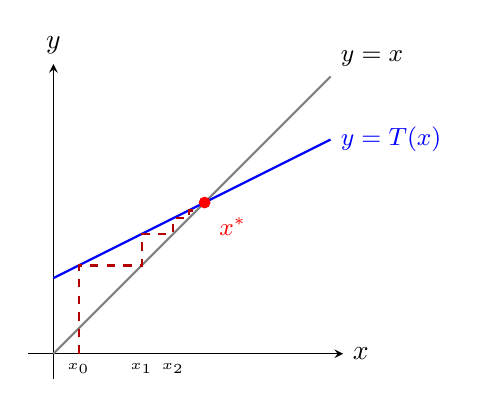
\begin{tikzpicture}[>=stealth, scale=3.2]
  % Axes
  \draw[->] (-0.1,0) -- (1.15,0) node[right] {$x$};
  \draw[->] (0,-0.1) -- (0,1.15) node[above] {$y$};
  % Line y = x
  \draw[thick, gray] (0,0) -- (1.1,1.1) node[above right, black] {\small $y = x$};
  % Function T (contraction): T(x) = 0.3 + 0.5x
  \draw[thick, blue, domain=0:1.1, samples=50] plot (\x, {0.3 + 0.5*\x})
    node[right] {\small $y = T(x)$};
  % Fixed point x* = 0.6
  \filldraw[red] (0.6,0.6) circle (0.6pt);
  \node[red, below right] at (0.62,0.58) {\small $x^*$};
  % Staircase iterates from x_0 = 0.1
  % x_0 = 0.1, T(x_0) = 0.35, T^2 = 0.475, T^3 = 0.5375, T^4 = 0.56875
  \draw[thick, dashed, red!70!black]
    (0.1,0) -- (0.1,0.35) -- (0.35,0.35) -- (0.35,0.475)
    -- (0.475,0.475) -- (0.475,0.5375) -- (0.5375,0.5375)
    -- (0.5375,0.56875) -- (0.56875,0.56875) -- (0.56875,0.584);
  % Labels
  \node[below] at (0.1,0) {\tiny $x_0$};
  \node[below] at (0.35,0) {\tiny $x_1$};
  \node[below] at (0.475,0) {\tiny $x_2$};
\end{tikzpicture}
\end{center}

\begin{keyformulas}[title=\textbf{Banach Contraction Principle}]
Let $(X, d)$ be complete, $T : X \to X$ with $d(Tx, Ty) \leq k \, d(x,y)$, $k < 1$. Then:
\[
    \exists!\, x^* \in X : T(x^*) = x^*, \qquad
    d(T^n x_0, x^*) \leq \frac{k^n}{1-k}\, d(x_0, Tx_0).
\]
\end{keyformulas}

\section{Necessity of hypotheses}

\begin{example}[Necessity of completeness]
Consider $X = (0, 1]$ with the usual metric and $T(x) = x/2$. Then $T$ is a
contraction with constant $1/2$, but $T$ has no fixed point in $X$ (the fixed
point $0$ does not belong to $X$). The space $(0,1]$ is not complete.
\end{example}

\begin{example}[Necessity of $k < 1$]
Let $X = [1, +\infty)$ with the usual metric and $T(x) = x + 1/x$. Then for
$x \neq y$:
\[
    \abs{T(x) - T(y)} = \abs{x - y} \cdot \abs{1 - \frac{1}{xy}} < \abs{x - y}
\]
so $T$ is weakly contractive ($d(Tx, Ty) < d(x,y)$ for $x \neq y$), but there
is no uniform $k < 1$. The map $T$ has no fixed point in $[1, +\infty)$.
\end{example}

\begin{warning}[title=\textbf{Strict contraction vs.\ weak contraction}]
The condition $d(Tx, Ty) < d(x,y)$ for $x \neq y$ (weak contraction) does
\textbf{not} suffice to guarantee existence of a fixed point, even in a complete
space. One needs the uniform condition $d(Tx, Ty) \leq k \, d(x,y)$ with $k < 1$
independent of $x$ and $y$.
\end{warning}

\section{Rate of convergence}

\begin{proposition}[Geometric convergence]
Under the hypotheses of Theorem~\ref{thm:banach}, the convergence of $(x_n)$ to
$x^*$ is at least geometric with ratio $k$:
\[
    d(x_n, x^*) \leq k \, d(x_{n-1}, x^*) \quad \forall n \geq 1.
\]
\end{proposition}

\begin{proof}
$d(x_n, x^*) = d(T(x_{n-1}), T(x^*)) \leq k \, d(x_{n-1}, x^*)$.
\end{proof}

\begin{remark}
In practice, the a posteriori estimate \eqref{eq:aposteriori} is more useful
because it does not require knowledge of $d(x_0, Tx_0)$ but only the last
variation $d(x_{n-1}, x_n)$, which is computed during the iteration.
\end{remark}

\section{Classical applications}

\subsection{Picard--Lindel\"of theorem}

\begin{theorem}[Picard--Lindel\"of]
Let $t_0 \in \R$, $y_0 \in \R^n$, and $f : [t_0 - a, t_0 + a] \times
\overline{B}(y_0, b) \to \R^n$ be continuous and Lipschitz in $y$ with constant
$L$. Set $M = \sup \norm{f}$ and $\delta = \min(a, b/M)$. If $L\delta < 1$,
then the Cauchy problem
\[
    y'(t) = f(t, y(t)), \quad y(t_0) = y_0
\]
has a unique solution on $[t_0 - \delta, t_0 + \delta]$.
\end{theorem}

\begin{proof}
Let $X = C([t_0 - \delta, t_0 + \delta], \overline{B}(y_0, b))$ with the
supremum norm. Define the Picard operator:
\[
    (Ty)(t) = y_0 + \int_{t_0}^t f(s, y(s)) \, ds.
\]
We verify that $T$ maps $X$ into $X$: for $y \in X$,
\[
    \norm{(Ty)(t) - y_0} \leq \int_{t_0}^t \norm{f(s, y(s))} \, ds \leq M\delta \leq b.
\]
We verify that $T$ is a contraction: for $y, z \in X$,
\[
    \norm{(Ty)(t) - (Tz)(t)} \leq \int_{t_0}^t L \, \norm{y(s) - z(s)} \, ds
    \leq L\delta \, \norm{y - z}_\infty.
\]
Since $L\delta < 1$, the Banach principle applies and provides existence and
uniqueness of the solution.
\end{proof}

\subsection{Fredholm integral equations}

\begin{theorem}[Fredholm equation]
Let $K \in C([a,b]^2)$ and $f \in C([a,b])$. If
$\abs{\lambda} \cdot \sup_{t} \int_a^b \abs{K(t,s)} \, ds < 1$, then the
equation
\[
    u(t) = f(t) + \lambda \int_a^b K(t,s) \, u(s) \, ds
\]
has a unique solution in $C([a,b])$.
\end{theorem}

\begin{proof}
The operator $(Tu)(t) = f(t) + \lambda \int_a^b K(t,s) u(s) \, ds$ is a
contraction on $(C([a,b]), \norm{\cdot}_\infty)$ with constant
$k = \abs{\lambda} \sup_t \int_a^b \abs{K(t,s)} \, ds < 1$.
\end{proof}

\subsection{Local inversion theorem}

\begin{theorem}[Local inversion via Banach]
Let $E$ be a Banach space and $F : E \to E$ be $C^1$ with $DF(x_0)$ invertible.
Then $F$ is a local diffeomorphism near $x_0$.
\end{theorem}

\begin{proof}[Proof sketch]
Without loss of generality, $x_0 = 0$ and $DF(0) = \mathrm{Id}$, so
$F(x) = x - \varphi(x)$ with $D\varphi(0) = 0$. For $y$ near $0$, the equation
$F(x) = y$ becomes $x = y + \varphi(x) = T_y(x)$. By continuity of $D\varphi$,
$T_y$ is a contraction on a sufficiently small ball around $0$.
\end{proof}

\section{Direct generalizations}

\subsection{Contractions on closed subsets}

\begin{proposition}[Contraction on a closed set]
Let $(X, d)$ be a complete metric space and $F \subset X$ a nonempty closed set.
If $T : F \to F$ is a contraction, then $T$ has a unique fixed point in $F$.
\end{proposition}

\begin{proof}
A closed subset of a complete space is complete, and we apply
Theorem~\ref{thm:banach}.
\end{proof}

\subsection{Contractive iterates}

\begin{theorem}[Contractive iterates]
Let $(X, d)$ be a complete metric space and $T : X \to X$ continuous. If $T^N$
is a contraction for some $N \geq 1$, then $T$ has a unique fixed point.
\end{theorem}

\begin{proof}
By Banach's theorem applied to $T^N$, there exists a unique $x^*$ with
$T^N(x^*) = x^*$. Then $T^N(T(x^*)) = T(T^N(x^*)) = T(x^*)$, so $T(x^*)$ is
also a fixed point of $T^N$. By uniqueness, $T(x^*) = x^*$.

Conversely, every fixed point of $T$ is a fixed point of $T^N$, so $T$ has a
unique fixed point.
\end{proof}

\begin{example}
The map $T : C([0,1]) \to C([0,1])$ defined by $(Tf)(x) = \int_0^x f(t) \, dt$
is not a contraction, but $T^N$ is a contraction for $N$ large enough since
$\norm{T^N f}_\infty \leq \frac{\norm{f}_\infty}{N!}$.
\end{example}

\subsection{Banach principle with parameter}

\begin{theorem}[Continuous dependence on a parameter]
Let $(X, d)$ be a complete metric space, $\Lambda$ a topological space, and
$T : X \times \Lambda \to X$ such that:
\begin{enumerate}
    \item For every $\lambda \in \Lambda$, $T(\cdot, \lambda)$ is a contraction
          with constant $k < 1$ (uniform in $\lambda$);
    \item For every $x \in X$, $T(x, \cdot) : \Lambda \to X$ is continuous.
\end{enumerate}
Then the map $\lambda \mapsto x^*(\lambda)$, where $x^*(\lambda)$ is the unique
fixed point of $T(\cdot, \lambda)$, is continuous.
\end{theorem}

\begin{proof}
Let $\lambda_0 \in \Lambda$ and $\varepsilon > 0$. We have:
\begin{align*}
    d(x^*(\lambda), x^*(\lambda_0))
    &= d(T(x^*(\lambda), \lambda), T(x^*(\lambda_0), \lambda_0)) \\
    &\leq d(T(x^*(\lambda), \lambda), T(x^*(\lambda_0), \lambda))
         + d(T(x^*(\lambda_0), \lambda), T(x^*(\lambda_0), \lambda_0)) \\
    &\leq k \, d(x^*(\lambda), x^*(\lambda_0))
         + d(T(x^*(\lambda_0), \lambda), T(x^*(\lambda_0), \lambda_0)).
\end{align*}
Hence $(1-k) \, d(x^*(\lambda), x^*(\lambda_0)) \leq
d(T(x^*(\lambda_0), \lambda), T(x^*(\lambda_0), \lambda_0))$. The right-hand
side tends to $0$ as $\lambda \to \lambda_0$ by hypothesis (2).
\end{proof}

\section{Generalized Banach--Caccioppoli theorem}

\begin{theorem}[Contraction on a ball]
Let $(X, d)$ be a complete metric space, $x_0 \in X$, $r > 0$, and
$T : \overline{B}(x_0, r) \to X$ a contraction with constant $k < 1$. If
\[
    d(x_0, T(x_0)) < (1 - k) r,
\]
then $T$ has a unique fixed point in $\overline{B}(x_0, r)$.
\end{theorem}

\begin{proof}
It suffices to show that $T(\overline{B}(x_0, r)) \subset \overline{B}(x_0, r)$.
For $x \in \overline{B}(x_0, r)$:
\[
    d(T(x), x_0) \leq d(T(x), T(x_0)) + d(T(x_0), x_0)
    \leq k \, d(x, x_0) + d(T(x_0), x_0) \leq kr + (1-k)r = r.
\]
Then apply Banach's theorem to $T : \overline{B}(x_0, r) \to \overline{B}(x_0, r)$.
\end{proof}

\section{Nonexpansive mappings}

\begin{definition}[Nonexpansive mapping]
A mapping $T : X \to X$ is \emph{nonexpansive} if $d(T(x), T(y)) \leq d(x, y)$
for all $x, y \in X$.
\end{definition}

\begin{remark}
A nonexpansive mapping need not have a fixed point, even in a complete space.
For example, the translation $T(x) = x + 1$ on $\R$ is nonexpansive with no
fixed point.
\end{remark}

\begin{theorem}[Browder--G\"ohde--Kirk, 1965]
Let $C$ be a bounded, closed, convex subset of a Hilbert space $H$. If
$T : C \to C$ is nonexpansive, then $T$ has a fixed point.
\end{theorem}

\begin{proof}[Proof sketch]
For $\lambda \in (0,1)$, fix $a \in C$ and define
$T_\lambda(x) = \lambda a + (1-\lambda) T(x)$. Then $T_\lambda$ is a contraction
with constant $1 - \lambda$ and maps $C$ into $C$ by convexity. Let $x_\lambda$
be its unique fixed point:
\[
    x_\lambda = \lambda a + (1-\lambda) T(x_\lambda).
\]
As $\lambda \to 0^+$, one shows (using the Hilbert space structure) that
$(x_\lambda)$ converges weakly to a fixed point of $T$.
\end{proof}

\section{Boyd--Wong generalized contractions}

\begin{theorem}[Boyd--Wong, 1969]
Let $(X, d)$ be a complete metric space and $T : X \to X$ satisfying
\[
    d(T(x), T(y)) \leq \psi(d(x, y)) \quad \forall x, y \in X,
\]
where $\psi : [0, \infty) \to [0, \infty)$ is upper semicontinuous from the
right and satisfies $\psi(t) < t$ for all $t > 0$. Then $T$ has a unique fixed
point.
\end{theorem}

\begin{proof}
Fix $x_0 \in X$ and set $x_n = T^n(x_0)$. The sequence $(d_n)$ defined by
$d_n = d(x_n, x_{n+1})$ is decreasing since $d_{n+1} \leq \psi(d_n) < d_n$
when $d_n > 0$. It therefore converges to a limit $\ell \geq 0$.

If $\ell > 0$, by upper semicontinuity from the right of $\psi$:
$\ell \leq \limsup_{n} \psi(d_n) \leq \psi(\ell) < \ell$, a contradiction.
Hence $\ell = 0$.

We show that $(x_n)$ is Cauchy. Argue by contradiction: there would exist
$\varepsilon > 0$ and subsequences $m(k) > n(k) \to \infty$ with
$d(x_{m(k)}, x_{n(k)}) \geq \varepsilon$. Choose $m(k)$ minimal, so
$d(x_{m(k)-1}, x_{n(k)}) < \varepsilon$. Then
\begin{align*}
    \varepsilon &\leq d(x_{m(k)}, x_{n(k)})
    \leq d(x_{m(k)}, x_{m(k)-1}) + d(x_{m(k)-1}, x_{n(k)})
    < d_{m(k)-1} + \varepsilon.
\end{align*}
So $d(x_{m(k)}, x_{n(k)}) \to \varepsilon$. By the contractive condition:
\[
    d(x_{m(k)+1}, x_{n(k)+1}) \leq \psi(d(x_{m(k)}, x_{n(k)})).
\]
Passing to the limit: $\varepsilon \leq \psi(\varepsilon) < \varepsilon$, a
contradiction. Hence $(x_n)$ is Cauchy.

By completeness, $x_n \to x^*$, and by continuity of $T$, $T(x^*) = x^*$.
Uniqueness follows as in Banach's theorem.
\end{proof}

\section{Meir--Keeler contractions}

\begin{theorem}[Meir--Keeler, 1969]
Let $(X, d)$ be a complete metric space and $T : X \to X$ satisfying: for every
$\varepsilon > 0$, there exists $\delta > 0$ such that
\[
    \varepsilon \leq d(x, y) < \varepsilon + \delta \implies d(T(x), T(y)) < \varepsilon.
\]
Then $T$ has a unique fixed point.
\end{theorem}

\begin{remark}
The Meir--Keeler condition implies $d(Tx, Ty) < d(x,y)$ for $x \neq y$ (take
$\varepsilon = d(x,y)$), but it is strictly stronger than a simple weak
contraction. Every Banach contraction (constant $k < 1$) satisfies the
Meir--Keeler condition with $\delta = \varepsilon(1-k)/k$.
\end{remark}

\section{Matkowski's fixed point theorem}

\begin{theorem}[Matkowski, 1975]
Let $(X, d)$ be a complete metric space and $T : X \to X$ satisfying
\[
    d(T(x), T(y)) \leq \psi(d(x, y)) \quad \forall x, y \in X,
\]
where $\psi : [0, \infty) \to [0, \infty)$ is increasing and satisfies
$\lim_{n \to \infty} \psi^n(t) = 0$ for all $t > 0$. Then $T$ has a unique
fixed point.
\end{theorem}

\begin{remark}
Note that if $\psi$ is increasing and $\psi^n(t) \to 0$, then $\psi(t) < t$
for all $t > 0$. Indeed, if $\psi(t_0) \geq t_0$ for some $t_0 > 0$, then by
monotonicity $\psi^n(t_0) \geq t_0$ for all $n$, contradicting $\psi^n(t_0) \to 0$.
\end{remark}

\section{Exercises}

\begin{exercise}
Let $T : \R \to \R$ be defined by $T(x) = \frac{1}{2}(x + a/x)$ for $x > 0$,
where $a > 0$. Show that for every $x_0 > 0$, the sequence $(T^n(x_0))$
converges to $\sqrt{a}$. Is this a Banach contraction?
\end{exercise}

\begin{exercise}
Show that the map $T : C([0,1]) \to C([0,1])$ defined by
$(Tf)(x) = \int_0^x f(t) \, dt$ is not a contraction, but $T^n$ is a
contraction for $n \geq 2$. Deduce that $T$ has a unique fixed point (the zero
function).
\end{exercise}

\begin{exercise}
Let $(X, d)$ be a complete metric space and $T : X \to X$ such that
$d(T(x), T(y)) \leq \alpha \, d(x, T(x)) + \beta \, d(y, T(y))$ with
$\alpha + \beta < 1$. Show that $T$ has a unique fixed point.
\textit{This is Kannan's condition, studied in Chapter~3.}
\end{exercise}

\begin{exercise}
Let $A$ be an $n \times n$ matrix with $\norm{A} < 1$ (operator norm). Show that
$(I - A)$ is invertible and $(I - A)^{-1} = \sum_{k=0}^\infty A^k$ (Neumann
series). Prove this using the Banach principle.
\end{exercise}

\begin{exercise}[Nadler's theorem]
Let $(X, d)$ be a complete metric space and $T : X \to \mathcal{K}(X)$ a
set-valued mapping with nonempty compact values that is contractive for the
Hausdorff metric:
\[
    H(T(x), T(y)) \leq k \, d(x, y), \quad k < 1.
\]
Show that $T$ has a fixed point, i.e., there exists $x^*$ with $x^* \in T(x^*)$.
\end{exercise}

\begin{exercise}
Let $f : \R^n \to \R^n$ be $C^1$ with $\norm{Df(x)} \leq k < 1$ for all $x$
(operator norm). Show that $f$ is a contraction and deduce that the equation
$x = f(x)$ has a unique solution.
\end{exercise}

\begin{exercise}
Study the convergence of Newton's method as a special case of the contraction
principle. Specifically, let $g : \R \to \R$ be $C^2$ with $g(x^*) = 0$ and
$g'(x^*) \neq 0$. Show that the iteration
$x_{n+1} = x_n - g(x_n)/g'(x_n)$ converges to $x^*$ for $x_0$ sufficiently
close to $x^*$, and that the convergence is quadratic.
\end{exercise}
